\documentclass[bachelor, och, labwork]{shiza}

\usepackage{subfigure}
\usepackage{tikz,pgfplots}
\pgfplotsset{compat=1.5}
\usepackage{float}

\usepackage{titlesec}
\setcounter{secnumdepth}{4}
\titleformat{\paragraph}
{\normalfont\normalsize}{\theparagraph}{1em}{}
\titlespacing*{\paragraph}
{35.5pt}{3.25ex plus 1ex minus .2ex}{1.5ex plus .2ex}

\titleformat{\paragraph}[block]
{\hspace{1.25cm}\normalfont}
{\theparagraph}{1ex}{}
\titlespacing{\paragraph}
{0cm}{2ex plus 1ex minus .2ex}{.4ex plus.2ex}

% --------------------------------------------------------------------------%


\usepackage[T2A]{fontenc}
\usepackage[utf8]{inputenc}
\usepackage{graphicx}
\graphicspath{ {./images/} }
\usepackage{tempora}

\usepackage[sort,compress]{cite}
\usepackage{amsmath}
\usepackage{amssymb}
\usepackage{amsthm}
\usepackage{fancyvrb}
\usepackage{listings}
\usepackage{listingsutf8}
\usepackage{longtable}
\usepackage{array}
\usepackage[english,russian]{babel}

\usepackage[colorlinks=true]{hyperref}
\usepackage{url}

\usepackage{underscore}
\usepackage{setspace}
\usepackage{indentfirst} 
\usepackage{mathtools}
\usepackage{amsfonts}
\usepackage{enumitem}
\usepackage{tikz}
\usepackage{minted}

\newcommand{\eqdef}{\stackrel {\rm def}{=}}
\newcommand{\specialcell}[2][c]{%
\begin{tabular}[#1]{@{}c@{}}#2\end{tabular}}

\renewcommand\theFancyVerbLine{\small\arabic{FancyVerbLine}}


\begin{document}

% \chair{Кафедра теоретических основ компьютерной безопасности и криптографии}

\title{Рекурсивные алгоритмы. Упр 3.2}

\course{3}

\group{331}

\department{факультета КНиИТ}

\napravlenie{10.05.01 "--- Компьютерная безопасность}

\author{Никитина Арсения Владимировича}

\satitle{доцент}

\saname{А. Н. Гамова}

\date{2022}

\maketitle

%-------------------------------------------------------------------------------
\tableofcontents

\intro
В данной работе будут рассмотрены принципы рекурсивных алгоритмов, в частности
алгоритма получения всех возможных перестановок элементов заданного множества
без использования дополнительной памяти.

\section{Постановка задачи}
Напишите процедуру формирования на том же местое всех $n!$ перестановок для $n$
элементов $a_1,...,a_n$, то есть без дополнительного массива. После формирования
очередной перестановки можно, например, обратиться к процедуре $Q$ (с параметром),
которая напечатает полученную перестановку.

Указание: задачу формирования всех перестановок элементов $a_1,...,a_m$ можно
считать состоящей из $m$ подзадач формирования всех перестановок для элементов
$a_1,...,a_{m-1}$, за которыми сделует $a_m$. Причем в $i$-й подзадаче вначале
меняются местами элементы $a_1 \text{и} a_m$

\section{Рекурсисный обьект}

\textit{Рекурсивным} называется объект, частично состоящий или определяемый с
помощью самого себя.

Мощность рекурсивного определения заключается в том, что оно позволяет с помощью
конечного высказывания определить бесконечное вычисление, причем программа не 
будет содержать явных повторений. Однако рекурсивные алгоритмы лучше всего
использовать, если в решаемой задаче, вычисляемой функции или структуре
обрабатываемых данных рекурсия уже присутствует явно. В общем виде рекурсивную
программу $P$ можно выразить как некоторую композицию $P$ из множества
операторов $S$ (не содержащих $P$) и самой $P$:
\begin{center}$P=P[S,P]$\end{center}

Для выражения рекурсивных программ необходимо и достаточно иметь понятие
процедуры или подрограммы, поскольку они позволяют дать любому оператору имя,
с помощью которого к нему можно обращаться. Если некоторая процедура $P$
содержит явную ссылку на саму себя, то ее называют \textit{прямо рекурсивной}.
Если же $P$ ссылается на другую процедуру $Q$, содержащую (прямую или косвенную)
ссылку на $P$, то $P$ называют \textit{косвенно рекурсивной}.

Подобно операторам цикла, рекурсивные процедуры могут приводить к
незаканчивающимся вычислениям, и, поэтому на эту проблему следует особо обратить
внимание. Очевидно основное требование, чтобы рекурсивное обращение к $P$
управлялось некоторым условием $B$, которое в какой-то момент становится ложным.


\subsection{Результаты тестирования программы}

        \begin{figure}[H]
            \centering
            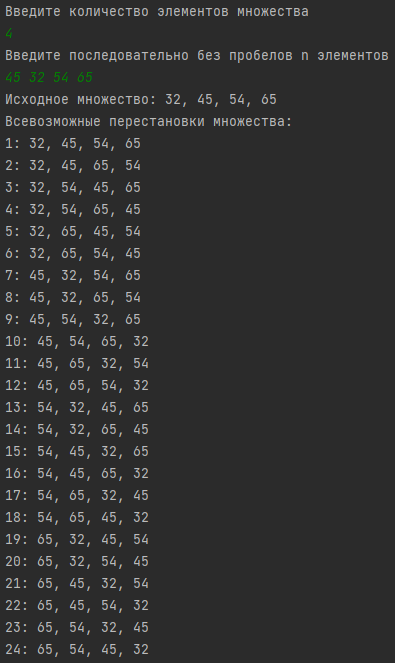
\includegraphics[width=0.8\textwidth]{1.png}
            \caption{}
        \end{figure}

\section{Программная реализация алгоритма}

\inputminted[linenos,breaklines=true, fontsize=\small, style=bw]{python}{1.py}

\section{Результаты работы программы}

\section{Оценка работы алгоритма}

Тут пока что пусто :)
% Для исследования производительности быстрой сортировки сначала необходимо
% разобраться, как идет процесс разделения. Выбрав некоторое граничное значение
% $x$, происходит обход по всему массиву, а, значит, при этом выполняется точно
% $n$ сравнений. Число же обменов можно определить из следующих
% вероятностных соображений.

% При заданной границе значений $x$ ожидаемое число операций обмена равно числу 
% элементов в левой части разделяемой последовательности, то есть $n-1$,
% умноженному на вероятность того, что при обмене каждый такой элемент перед этим
% находился в правой части. Вероятность этого равна $(n-(x-1))/n$. Поэтому 
% ожидаемое число обменов есть среднее этих ожидаемых значений для возможных
% границ, то есть получаем: $((n-1)/n)/6$.

% Пусть всегда удается выбрать в качестве границы медиану, в этом случае каждый 
% процесс разделений ресщеплет массив на две половины и для сортировки требуется
% всего $\log n$ проходов. В результате общее число сравнений равно $n*\log n$,
% а общее число обменов - $n * \log (n)/6$.

% Если же выбор разделяющего элемента не всегда идеален, то сложность алгоритма
% отличается на коэффициент $2* \ln 2$.

% Также стоит сказать, что алгоритм имеет преимущетсво перед другими
% усовершенствованными, что для обработки небольших частей массива в него можно 
% включить какой-либо из методом прямой сортировки.

% Наихудший же случай работы алгоритма достигается, когда для сравнения выбирается
% наибольший элемент из значений, сосоящих в части. Тогда на каждом этапе сегмент 
% из $n$ элементов будет расщепляться на левую часть, состоящую из $n-1$ элементов,
% и на правую часть, состоящую из одного элемента (выбранного). Тогда в результате
% требуется $n$ разделений и наихудшая произовительность метода будет порядка 
% $n^2$. 

% Исследования Сама Хоара показывают, что наилучшая производительность алгоритма
% достигается при случайном выборе разделяющего элемента.

\conclusion

Тут тоже..
% Итак, в данной работе был рассмотрен алгоритм сортировки с помощью разделения.
% Произведена оценка его работы в худшем и в лучшем случае. В худшем случае
% ассимптотика работы алгоритма составляет $O(n^2)$ операций, 
% в лучшем - $O(n*\log n)$.

% Наиболее оптимальмальная работа алгоритма достигается при случайном выборе
% разделяющего элемента: в таком случае вероятность того, что за один проход
% алгоритма будет совершено операций обмена менее $\log n$ при 
% $\lim\limits_{n\rightarrow\infty }$ стремится к нулю.
\end{document}